	\documentclass[%
oneside,                 % oneside: electronic viewing, twoside: printing
final,                   % draft: marks overfull hboxes, figures with paths
10pt]{article}

\listfiles               %  print all files needed to compile this document


\usepackage[totoc]{idxlayout}   % for index in the toc
\usepackage[nottoc]{tocbibind}  % for references/bibliography in the toc

\usepackage{relsize,makeidx,color,setspace,amsmath,amsfonts,amssymb}
\usepackage[table]{xcolor}
\usepackage{bm,ltablex,microtype}
\usepackage{comment} 
\usepackage[pdftex]{graphicx}

\usepackage{fancyvrb} % packages needed for verbatim environments

\usepackage[T1]{fontenc}
%\usepackage[latin1]{inputenc}
\usepackage{ucs}
\usepackage[utf8x]{inputenc}

\usepackage{lmodern}         % Latin Modern fonts derived from Computer Modern


\usepackage{pgfplotstable, booktabs}

\pgfplotstableset{
    every head row/.style={before row=\toprule,after row=\midrule},
    every last row/.style={after row=\bottomrule}
}





% Hyperlinks in PDF:
\definecolor{linkcolor}{rgb}{0,0,0.4}
\usepackage{hyperref}
\hypersetup{
    breaklinks=true,
    colorlinks=true,
    linkcolor=linkcolor,
    urlcolor=linkcolor,
    citecolor=black,
    filecolor=black,
    %filecolor=blue,
    pdfmenubar=true,
    pdftoolbar=true,
    bookmarksdepth=3   % Uncomment (and tweak) for PDF bookmarks with more levels than the TOC
    }
%\hyperbaseurl{}   % hyperlinks are relative to this root

\setcounter{tocdepth}{2}  % levels in table of contents

% --- fancyhdr package for fancy headers ---
\usepackage{fancyhdr}
\fancyhf{} % sets both header and footer to nothing
\renewcommand{\headrulewidth}{0pt}
\fancyfoot[LE,RO]{\thepage}
% Ensure copyright on titlepage (article style) and chapter pages (book style)
\fancypagestyle{plain}{
  \fancyhf{}
  \fancyfoot[C]{{\footnotesize \copyright\ 1999-2018, "Computational Physics I FYS3150/FYS4150":"http://www.uio.no/studier/emner/matnat/fys/FYS3150/index-eng.html". Released under CC Attribution-NonCommercial 4.0 license}}
%  \renewcommand{\footrulewidth}{0mm}
  \renewcommand{\headrulewidth}{0mm}
}
% Ensure copyright on titlepages with \thispagestyle{empty}
\fancypagestyle{empty}{
  \fancyhf{}
  \fancyfoot[C]{{ }}
  \renewcommand{\footrulewidth}{0mm}
  \renewcommand{\headrulewidth}{0mm}
}

\pagestyle{fancy}


% prevent orhpans and widows
\clubpenalty = 10000
\widowpenalty = 10000

% --- end of standard preamble for documents ---


% insert custom LaTeX commands...

\raggedbottom
\makeindex
\usepackage[totoc]{idxlayout}   % for index in the toc
\usepackage[nottoc]{tocbibind}  % for references/bibliography in the toc
\usepackage{listings}
\usepackage[normalem]{ulem} 	%for tables
\useunder{\uline}{\ul}{}
\usepackage{hyperref}
\usepackage[section]{placeins} %force figs in section

\usepackage{natbib}


%-------------------- end preamble ----------------------

\begin{document}

% matching end for #ifdef PREAMBLE

\newcommand{\exercisesection}[1]{\subsection*{#1}}


% ------------------- main content ----------------------



% ----------------- title -------------------------

\thispagestyle{empty}

\begin{center}
{\LARGE\bf
\begin{spacing}{1.25}
MAT3110, Autumn 2019, Compulsory
assignment 1
\end{spacing}
}
\end{center}

% ----------------- author(s) -------------------------

\begin{center}
{\bf Johan Nereng}
\end{center}

    \begin{center}
% List of all institutions:
\centerline{{\small Department of Physics, University of Oslo, Norway}}
\end{center}
    
% ----------------- end author(s) -------------------------

% --- begin date ---
\begin{center}
Sep 25, 2019
\end{center}
% --- end date ---

\vspace{5cm}
\newpage
\section{Least Squares of a polynomial fit}
This assignment focuses on minimizing the sum of squares, $S$, of errors from a polynomial fit of degree $m$ to a data set $\{x_i,y_i\} _{i=1}^n$. From this data set, a Vandermonde matrix
\begin{equation}
A=\begin{bmatrix}
    1       & x_1 & x_1^2 & \dots & x_1^{m-1} \\
    2       & x_2 & x_2^2 & \dots & x_2^{m-1} \\
    \hdotsfor{5} \\
    n       & x_n & x_3^2 & \dots & x_n^{m-1}
\end{bmatrix}
\end{equation}
corresponding to the choice of $m$ may be constructed, along with a vector $\mathbf{x} =[c_1,c_2, \dots,c_m]$, containing the coefficients of the polynomial. If $\mathbf{b}=[y_1,y_2,\dots,y_n]$, then $S=\sum_{i=1}^n (p(x)-y_i)$ may be expressed as $S=||A\bf x - \bf b ||^2_2$. In order to minimize $S$, this assignment utilizes two methods: a QR factorization of $A$, and solving the normal equations $A^TAx=A^Tb$ using Cholesky factorization and forward substitution.

\subsection{Solving Least Squares with QR factorization}
Assuming that the Vandermonde matrix $A$ described earlier has linearly independent columns, it may be factorized as $QR=A$, where $Q$ is an orthogonal ${\Bbb R}^n$ matrix and $R$ an  upper ${\Bbb R}^n$ triangular matrix \cite{MF3}. Additionally, and generally, the  vector $\bf x \in {\Bbb R}^m$ minimizes $||A\bf x - \bf b||$ IFF it minimizes $||\Omega A \bf x - \bf b||$ for any orthogonal  matrix $\Omega$ \cite{MF4}. Using this, the minimization
\begin{equation}
||A\mathbf{x} - \mathbf{b} ||^2 = ||Q^TA\mathbf{x}-Q^T\mathbf{b}||^2=||R\mathbf{x}-Q^T\mathbf{b}||^2=||\begin{bmatrix} R_1 \\ 0 \end{bmatrix} \mathbf{x}-\begin{bmatrix} c_1 \\ c_2 \end{bmatrix}||^2
\end{equation} 
Thus solving the minimization corresponds to solving $R_1 \mathbf{x} = c_1$, which, since $R_1$ is a non-singular, upper triangular matrix, may be accomplished by backward substitution.

\subsection{Solving Least Squares with Cholesky factorization and forward substitution}
An alternative method for obtaining the coefficients in $\mathbf{x}$ is solving the normal equations using a Cholesky factorization. The 2-norm is a convex function, with a unique minimum. This minimum is found by taking the gradient of the norm, which leads to the normal equation:
\begin{equation}
A^TA\mathbf{x}=A^t\mathbf{b}
\label{eq:norm}
\end{equation}
The matrix $B=A^TA$ is a symmetric $n\times n$ matrix, which allows the application of the Cholesky factorization \cite{MF3}: $B=R^TR$, where $R \in {\Bbb R}^n$ is a lower triangular matrix. Thus \eqref{eq:norm} may be written as $RR^T\mathbf{x}=A^T\mathbf{b}$. In order to solve for $\mathbf{x}$, define $R^T \mathbf{x}=\mathbf{w}$, and solve $R\mathbf{w}=A^T\mathbf{b}$ for $\mathbf{w}$ by forward substitution. $R^T \mathbf{x}=\mathbf{w}$ is then solved  by backward substitution.
 
\section{Method implementation}
Algorithms \cite{MF3} \cite{MF4} for solving the Least Squares fit is implemented using both QR factorization and forward substitution, and Cholesky factorization with forward and backward substitution. For the purpose of this assignment, Python 3.7 using the Numpy library was used. Following the guidelines provided by the professor in class, the code is not included in this assignment. 

\subsection{Functions for testing the implementation}
In order to test the implementation, two function were employed: 
\begin{align}
f_1(x)&= x (cos(r+0.5x^3)+sin(0.5x^3)) \\
f_2(x)& = 4x^5- 5x^4 - 20x^3 + 10x^2 + 40x + 10 + r
\end{align}
where $r=\mathit{U}(0,1)$.  

\subsection{Application of methods to test functions}
Fitting of polynomials of degree $m=3$ and $m=8$, using both $f_1(x)$ and $f_2(x)$ for $x\in[-2,2]$, are displayed in figure \ref{fig:methods}. In the plots, the two methods are indistinguishable, indicating similar fitting. At the same time, it is evident that they polynomials do not match the data completely. This is to be expected, as the original functions are trigonometric, which cannot be approximated by $m$ degree polynomials. By-eye evaluation of the polynomials do however suggest that the methods were successfully implemented. More in-depth evaluation could be done using MSE or $R^2$, but such evaluation measurements were not used for the purpose of this assignment.

\begin{figure}[!htb]
        \centering 
         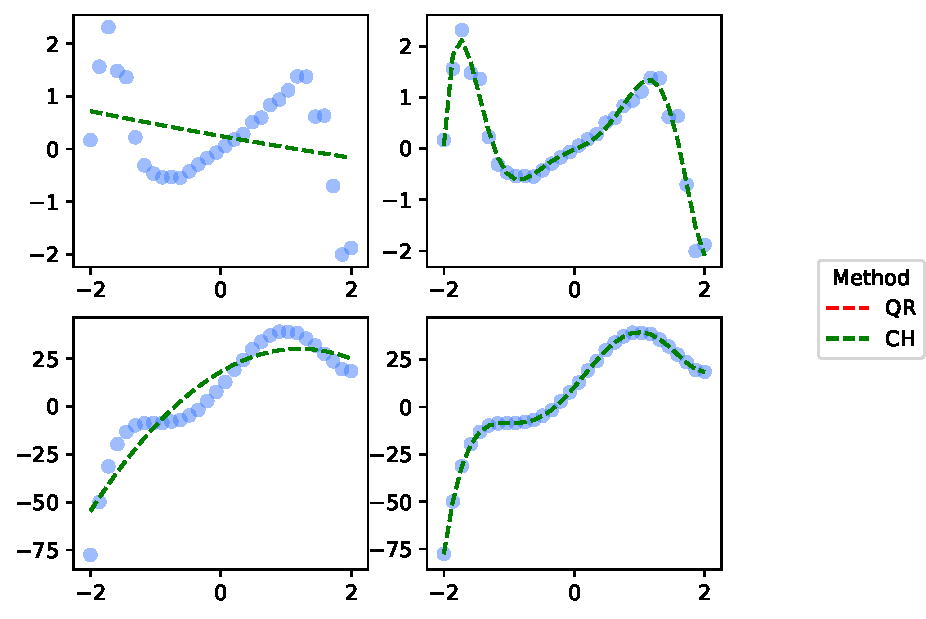
\includegraphics[scale=0.8]{Figures/methods.pdf} 
        \caption{Plot of polynomial fitting of degree $m=3$ (left column), and $m=8$ (right column), to $f_1(x)$ (upper row), and $f_2(x)$ (bottom row) using both QR and Cholesky (CH)}
        \label{fig:methods}   
\end{figure}  
\section{Method comparison}
\subsection{Computational Cost}
The two applied fitting methods are dissimilar in computational cost, measured in floating point operations (flops) - especially in the case where $m<<n$. The normal equation solution uses $mn^2
+ (1/3)n^3$ flops \citep{Ascher}[p.146], while the QR decomposition requires $2mn^2−(2/3)n^3$ flops  \citep{Ascher}[p.155]. Which means that the normal equations method is significantly faster than the QR approach.

\subsection{Conditioning}
The conditioning of the methods, or stability with respect to input perturbation, are measured in conditioning number of the matrix representing the problem, $K(A)$. Higher $K(A)$ means less stable. 
\begin{equation}
K(A)=||A^{-1}|| \times ||A||
\end{equation}
In order to acquire the normal equations, the product of $A$ and it's transpose is used. Hence, it's conditioning number goes as $K(A^TA)=K(A)^2$. This squaring of the conditioning number is not required for the QR approach, which means that the QR method has a lower conditioning number, and is thus the more stable method.

\section{Conclusions}
When handling well-conditioned Vandermonde matrices, the normal equations solution with Cholesky is faster than the QR method, and not necessarily particularly unstable. However, the larger the Vanermonde matrix is, the less well-conditioned it becomes. For higher order fittings, one may therefor expect the normal equations approach to be less well suited, as the solution will tend towards instability. On the other hand, the QR method is stable for a much larger variety of problems, and should therefor be employed when the polynomial degree (or number of predictors) is large. 


\bibliography{ref}
\bibliographystyle{plain}

\end{document}